\documentclass[11pt,a4paper]{article}

\usepackage[spanish,es-nodecimaldot]{babel}
\usepackage[T1]{fontenc}
\usepackage[utf8]{inputenc}
\usepackage{lmodern}
\usepackage{geometry}
\usepackage{graphicx}
\usepackage{float}
\usepackage{hyperref}
\usepackage{enumitem}
\usepackage{array}
\usepackage{amsmath}
\usepackage{longtable}

\geometry{margin=2.5cm}
\hypersetup{colorlinks=true,linkcolor=black,urlcolor=blue}
\graphicspath{{img/}{openssl_lab/evidence/screenshots/}}

\title{Criptografía y certificados digitales con OpenSSL}
\author{Javier Siñuka}
\date{13 de octubre de 2026}

\begin{document}
\maketitle

\begin{abstract}
Se realizaron pruebas locales de cifrado simétrico, cifrado RSA y cifrado
híbrido con OpenSSL, además de una práctica aislada de HTTPS y ACME mediante
Apache, Certbot y Pebble en contenedores Docker. Las comparaciones byte a byte
y SHA-256 verificaron los descifrados correctos; las pruebas negativas
mostraron el rechazo de una clave RSA incorrecta, el error con una contraseña
simétrica errónea y la ausencia de autenticación en AES-CBC. Se obtuvo y sirvió
un certificado de una CA ACME de prueba, y se verificaron su nombre, cadena y
raíz. No se emitió un certificado de Let's Encrypt: no se dispone de un dominio
propio ni de acceso a su DNS. La práctica local reproduce aspectos del flujo
ACME, pero no equivale a una emisión pública. Se incorporan capturas reales de
Chromium mostrando el directorio ACME de Pebble y la página servida por Apache
con el certificado emitido localmente, además de capturas de las pruebas
criptográficas ejecutadas en una VM Ubuntu aislada.
\end{abstract}

\noindent\textbf{Palabras clave:} OpenSSL, AES, RSA, cifrado híbrido, X.509, PKI,
ACME, HTTPS.

\section{Objetivo}
Completar las actividades de cifrado simétrico, asimétrico e híbrido de la guía
de OpenSSL; explicar los fundamentos de X.509 y las Autoridades de
Certificación; y practicar la emisión ACME, el despliegue HTTPS y la
verificación de una cadena en un entorno local aislado. Se distinguen los
resultados efectivamente observados de los requisitos públicos que no pueden
validarse sin un dominio controlado.

\section{Material y metodología}
Se utilizaron las guías \emph{Práctica de laboratorio: Cifrar y descifrar
datos con OpenSSL} (9 páginas) y \emph{Criptografía y Certificados Digitales
en la Práctica} (2 páginas). Las pruebas criptográficas se ejecutaron en
Ubuntu 24.04.5 LTS con OpenSSL 3.0.13. Para HTTPS se ejecutaron Apache 2.4.69,
Certbot 5.8.0 y Pebble en contenedores Docker; Docker fue 29.8.2 y Docker
Compose 5.6.0. Los puertos publicados se vincularon a \texttt{127.0.0.1}; no
se alteraron DNS públicos, el firewall, el almacén de confianza del sistema ni
servicios web del host.

Los archivos de trabajo, scripts y salidas están bajo \path{openssl_lab/}.
Las frases de prueba, claves privadas y el material secreto se guardaron como
archivos de laboratorio con permisos restrictivos y se excluyeron de las
capturas. Las dos primeras imágenes son capturas reales, sin editar, de la
consola de una VM desechable Ubuntu 24.04.5 LTS con OpenSSL 3.0.13. Las dos
últimas son capturas del navegador Chromium al consultar el endpoint ACME de
Pebble y el sitio HTTPS de Apache. Para esta última se agregó la raíz Pebble
sólo al perfil temporal del navegador; no se modificó el almacén del sistema.
La consulta visual al directorio ACME aceptó el certificado TLS de prueba de
Pebble, por lo que esa imagen documenta la respuesta ACME y no la confianza de
su certificado de servidor.

\section{Evidencia gráfica}
\begin{figure}[H]
\centering
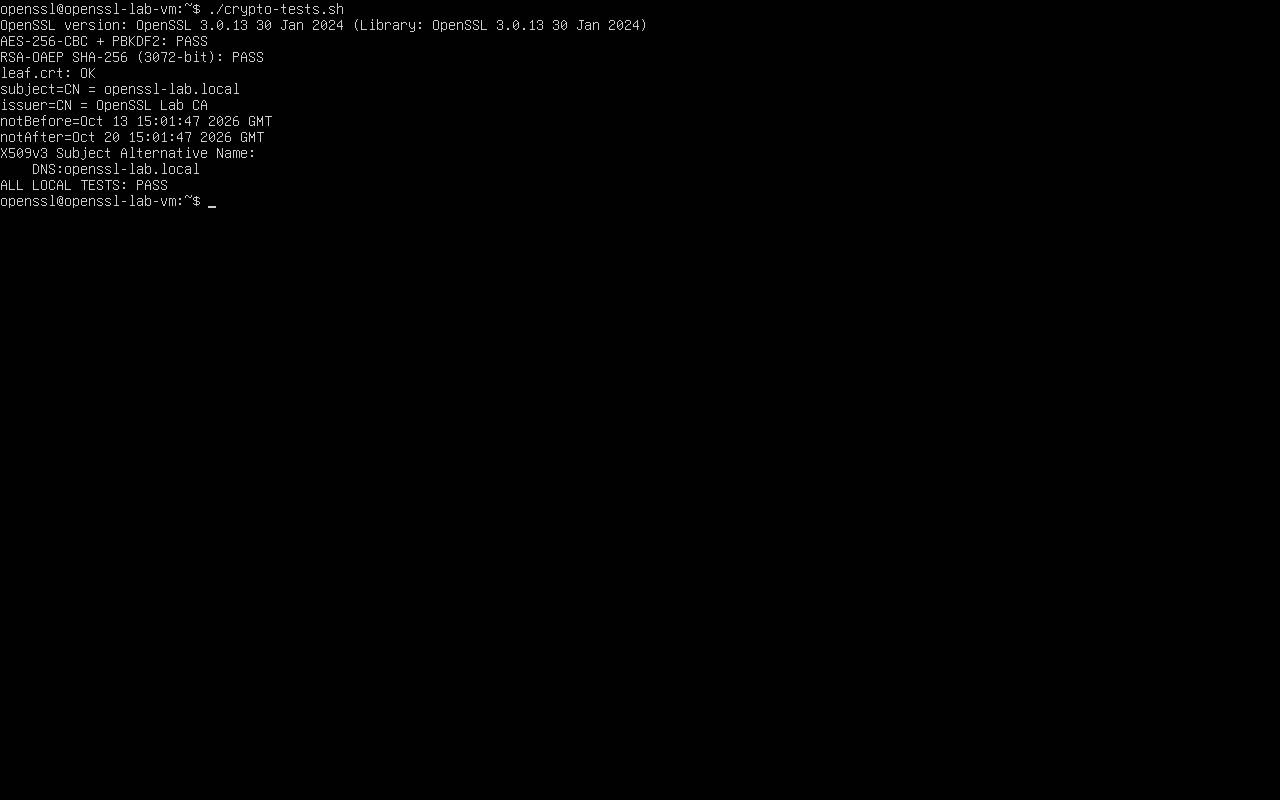
\includegraphics[trim=0cm 20.46cm 16.93cm 0cm,clip,width=0.96\textwidth,height=0.57\textheight,keepaspectratio]{01-pruebas-criptograficas-vm.png}
\caption{Captura real de la consola Ubuntu: OpenSSL 3.0.13, descifrado AES-256-CBC con PBKDF2 confirmado por \texttt{cmp}, RSA-OAEP-SHA256 confirmado por comparación byte a byte y validación del certificado local.}
\label{fig:vm-crypto}
\end{figure}

\begin{figure}[H]
\centering
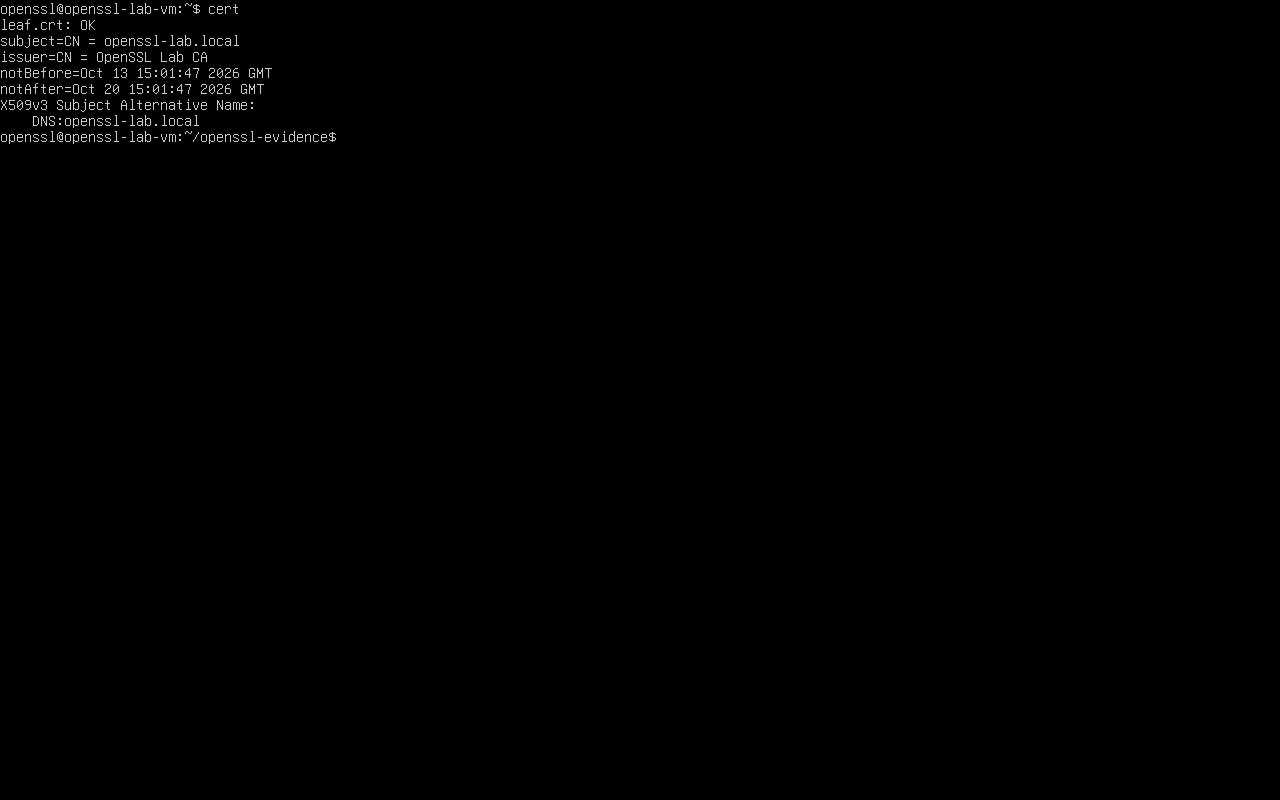
\includegraphics[trim=0cm 21.87cm 16.93cm 0cm,clip,width=0.96\textwidth,height=0.57\textheight,keepaspectratio]{02-verificacion-certificado-vm.png}
\caption{Captura real de la verificación del SAN \texttt{openssl-lab.local}, emisor y vigencia del certificado de laboratorio con \texttt{openssl verify} y \texttt{openssl x509}. La CA de esta imagen es local y no es Pebble ni Let's Encrypt.}
\label{fig:vm-x509}
\end{figure}

\begin{figure}[H]
\centering
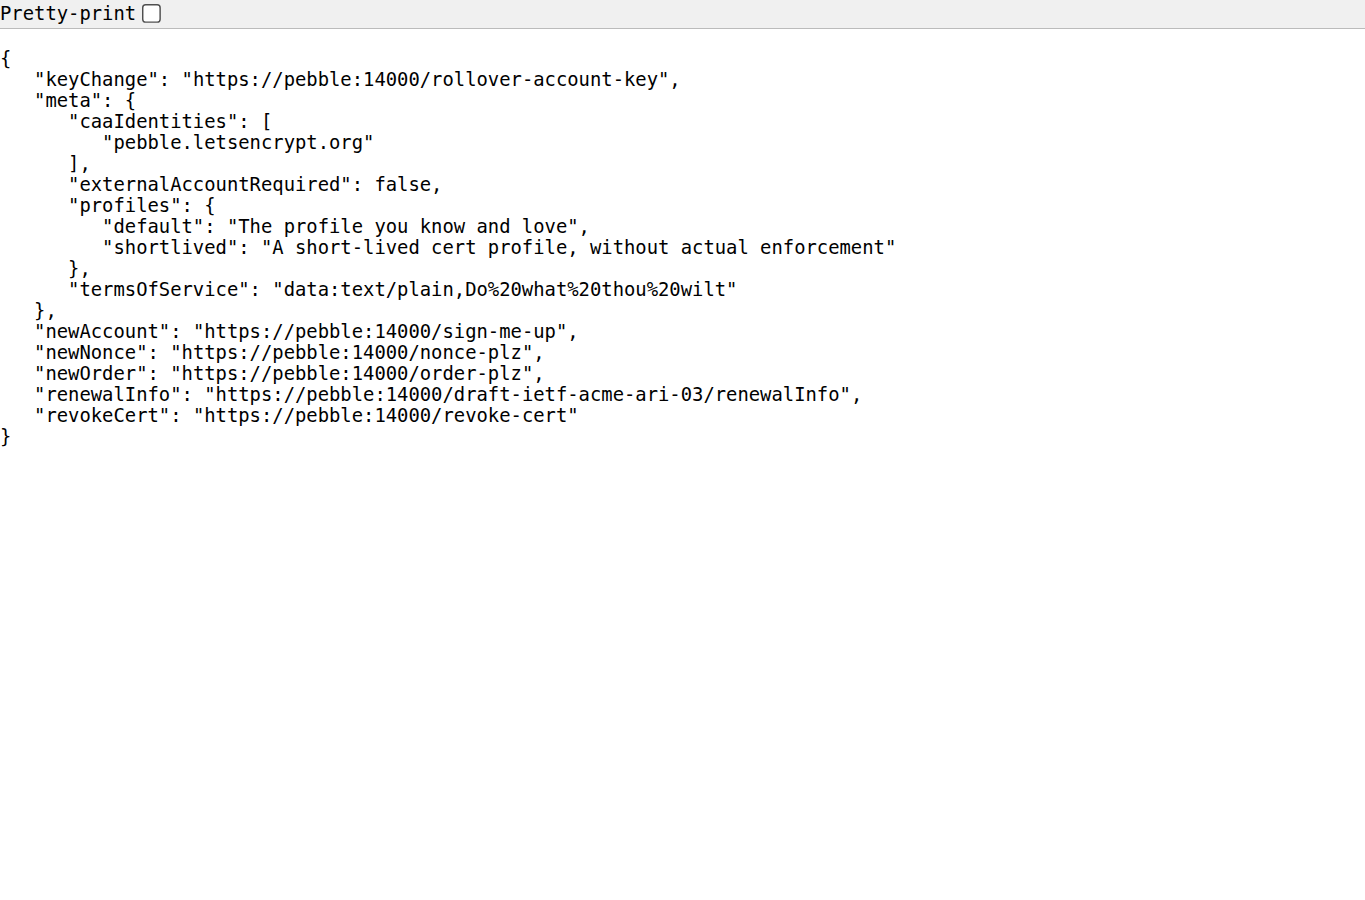
\includegraphics[trim=0cm 12cm 8cm 0.5cm,clip,width=0.94\textwidth,height=0.42\textheight,keepaspectratio]{04-directorio-acme-pebble-chromium.png}
\caption{Chromium muestra la respuesta HTTP 200 del directorio ACME local de Pebble. La sesión aceptó el certificado TLS de prueba; la captura no demuestra confianza pública ni emisión de Let's Encrypt.}
\label{fig:pebble-directory}
\end{figure}

\begin{figure}[H]
\centering
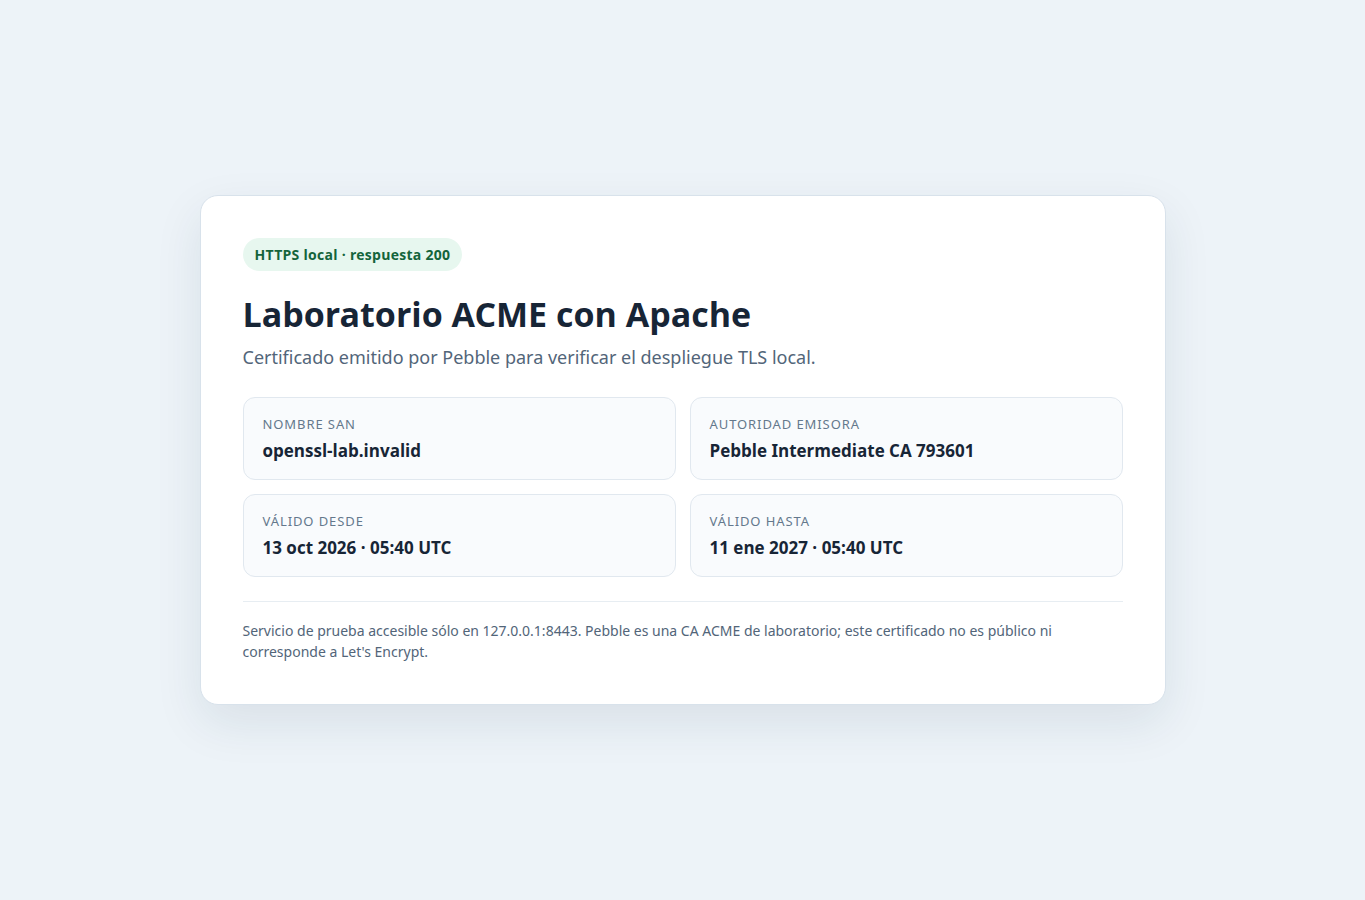
\includegraphics[trim=5cm 5cm 5cm 5cm,clip,width=0.94\textwidth,height=0.42\textheight,keepaspectratio]{03-apache-https-chromium.png}
\caption{Chromium muestra Apache HTTPS en \texttt{openssl-lab.invalid:8443} con respuesta HTTP 200. La raíz Pebble se confió sólo en el perfil temporal de captura.}
\label{fig:apache-browser}
\end{figure}

\section{Fundamentos teóricos}
\subsection{Cifrado simétrico, AES-CBC y derivación de claves}
La criptografía simétrica cifra y descifra con un secreto compartido. AES
procesa bloques de 128 bits y CBC encadena cada bloque con el anterior mediante
un vector de inicialización. CBC no autentica el ciphertext: una modificación
puede producir texto alterado sin que el descifrado detecte necesariamente la
manipulación. Para datos sensibles se requiere un esquema autenticado, por
ejemplo AES-GCM, o una construcción que combine cifrado y autenticación de
manera correcta.

Cuando se proporciona una contraseña a \texttt{openssl enc}, OpenSSL deriva
una clave y un vector de inicialización. La modalidad heredada empleada por la
guía provocó la advertencia \texttt{deprecated key derivation}; la opción
\texttt{-pbkdf2} con parámetros iguales al cifrar y descifrar es una mejora
respecto de esa derivación. La sal aleatoria evita reutilizar directamente la
misma derivación para una contraseña en cada cifrado, pero no convierte una
contraseña débil en una clave segura.

Base64 transforma bytes en una representación textual. Facilita el transporte
en canales que esperan caracteres imprimibles, pero no es cifrado, no agrega
confidencialidad y aumenta el tamaño del contenido.

\subsection{RSA y cifrado híbrido}
En RSA, la clave pública puede difundirse y la privada debe permanecer
confidencial. Alice puede cifrar para Bob con la clave pública de Bob; sólo la
clave privada correspondiente puede descifrar. La operación no autentica por
sí sola quién generó el ciphertext: para vincular una clave pública con una
identidad se requiere una firma, un certificado u otro canal autenticado.

RSA sólo admite mensajes de tamaño acotado por el módulo y el relleno. Con una
clave RSA de 3072 bits y OAEP con SHA-256, el tamaño máximo teórico del mensaje
es \(384-2(32)-2=318\) bytes. Para archivos grandes se cifra el archivo con
una clave simétrica aleatoria y se protege únicamente esa clave con RSA.

\subsection{Certificados X.509 y confianza}
Un certificado X.509 contiene una clave pública, información del sujeto,
período de validez, usos y extensiones, junto con una firma de una CA. El
cliente construye una ruta desde el certificado final hasta un ancla presente
en su almacén de confianza. La firma verifica la integridad y la procedencia
del certificado respecto de la clave del emisor; la validación completa
incluye además nombre del servidor, vigencia, restricciones de CA, usos y,
según política y cliente, estado de revocación~\cite{rfc5280}.

La raíz suele ser autofirmada y sus claves se mantienen bajo controles
reforzados. Las CA intermedias firman certificados de uso operativo. Las CRL
publican certificados revocados; OCSP permite consultar su estado. Son
relevantes antes del vencimiento porque un certificado puede dejar de ser
confiable tras una filtración de clave o una emisión indebida. Los clientes
pueden aplicar estas comprobaciones de forma distinta, por disponibilidad,
políticas de privacidad, uso de caché o mecanismos de revocación propios
\cite{rfc5280,rfc6960}.

\section{Pruebas de criptografía simétrica}
\subsection{E01: carta de prueba}
Se creó el texto de la guía con la referencia al pan casero con chicharrones y
al salame de Colonia Caroya. El archivo es UTF-8, tiene 240 bytes y su
SHA-256 es \texttt{ce826f3b0089e4b8\allowbreak f8571a23031a2bda\allowbreak f8601033df1dbba7\allowbreak 82410c00fa487aa7}.
El contenido se inspeccionó con \texttt{cat}; se verificaron por separado el
tamaño del archivo y su huella SHA-256.

\subsection{E02 y E03: AES-256-CBC binario y Base64}
Se cifró la carta en la forma indicada por la guía, usando una frase aleatoria
de demostración que no se publica. OpenSSL emitió la advertencia de derivación
heredada. El archivo binario resultó de 272 bytes y comenzó con la cabecera
\texttt{Salted\_\_}; su contenido se inspeccionó mediante \texttt{xxd}. La
versión codificada con \texttt{-a} midió 370 bytes y fue reconocida por
\texttt{file} como salida Base64 de \texttt{openssl enc}. La ventaja práctica
de Base64 es poder transportar bytes cifrados en sistemas textuales; no agrega
seguridad.

\begin{verbatim}
openssl aes-256-cbc -in letter_to_grandma.txt -out message_binary.enc
openssl aes-256-cbc -a -in letter_to_grandma.txt -out message_base64.enc
\end{verbatim}

En la ejecución automatizada se utilizó además \texttt{-pass file:...} para
que la frase no quedara visible en el historial de la shell ni en la salida
visible. Este ajuste cambia la forma de introducir la frase, no el algoritmo
ni la transformación AES-CBC exigida.

\subsection{E04: descifrado y pruebas negativas}
La opción \texttt{-a} se utiliza al descifrar porque la entrada está codificada
en Base64 y debe decodificarse antes de descifrarla. La salida descifrada
coincidió byte a byte con la carta original; ambos SHA-256 fueron idénticos.
Con una frase incorrecta, OpenSSL informó error de descifrado. Ese fallo suele
derivarse de un padding inválido y no constituye un mecanismo de autenticación
robusto.

También se alteró un byte del ciphertext AES-CBC. OpenSSL terminó el
procesamiento y el archivo restaurado no coincidió con el original. El
resultado demuestra que CBC sin autenticación no garantiza integridad; un
error de padding puede ocurrir, pero no es seguro confiar en él como detector
de modificaciones.

\section{Pruebas de criptografía asimétrica}
\subsection{E05: pares de Alice y Bob}
Se generaron pares RSA de 3072 bits con claves privadas cifradas y se
extrajeron sus claves públicas. Las claves privadas tuvieron permisos
\texttt{rw-------} (0600). OpenSSL informó \texttt{Private-Key: (3072 bit,
2 primes)} al inspeccionar sus metadatos; no se volcó ningún componente
privado. El archivo público pudo compartirse sin comprometer el secreto
privado.

La guía emplea RSA-1024 y el comando \texttt{rsautl}; ambos son históricos.
Para la prueba actual se usó \texttt{pkeyutl} y relleno RSA-OAEP con SHA-256,
indicando también SHA-256 para MGF1.

\subsection{E06: mensajes en ambas direcciones}
El archivo solicitado \texttt{top\_secret.txt} contuvo exactamente
\texttt{vim or emacs ?} (14 bytes). Alice lo cifró con la clave pública de
Bob; Bob lo descifró con la clave privada propia y \texttt{cmp} devolvió
coincidencia. El ciphertext RSA midió 384 bytes, igual al tamaño del módulo
RSA-3072. El intento con la clave privada de Alice fue rechazado. Bob cifró
luego el mensaje de respuesta con la clave pública de Alice y ella lo recuperó
con éxito.

\begin{verbatim}
openssl pkeyutl -encrypt -pubin -inkey bob_public.pem \
  -in top_secret.txt -out top_secret.enc \
  -pkeyopt rsa_padding_mode:oaep \
  -pkeyopt rsa_oaep_md:sha256 -pkeyopt rsa_mgf1_md:sha256
\end{verbatim}

El éxito confirma confidencialidad frente a quien no tiene la clave privada,
pero no autentica a Alice ni a Bob. Si un atacante reemplaza la clave pública
intercambiada, puede hacerse pasar por una de las partes. El intercambio debe
validarse mediante certificados, huellas por un canal autenticado u otro
mecanismo equivalente.

\section{Prueba de cifrado híbrido}
\subsection{E07: archivo grande y recuperación}
Se generó un archivo determinista de 2 MiB (2\,097\,152 bytes) repitiendo la
secuencia de bytes de 0 a 255. Su SHA-256 fue
\texttt{91d3beb88a9b2f77\allowbreak 8a6c44a1c53b63d3\allowbreak c79931845a9aef84\allowbreak b3fb414610bd1938}.
Se generó una frase aleatoria de alta entropía en hexadecimal, se cifró el
archivo con AES-256-CBC y PBKDF2 de 200\,000 iteraciones y se cifró esa frase
exacta con la clave pública de Bob usando RSA-OAEP-SHA256. Bob recuperó la
frase con su clave privada y descifró el archivo usando los mismos parámetros
PBKDF2. \texttt{cmp} y SHA-256 confirmaron una restauración idéntica.

La adaptación corrige dos ambigüedades de la guía: \texttt{-k key.bin}
interpreta \texttt{key.bin} como una contraseña literal, no como una ruta cuyo
contenido se lea; y el descifrado debe repetir PBKDF2 y sus parámetros. Aquí
se usó \texttt{-pass file:...} para leer el secreto desde un archivo protegido,
y el mismo valor fue el material cifrado con RSA. El archivo cifrado midió
2\,097\,184 bytes; el secreto protegido por RSA, 384 bytes.

\begin{figure}[H]
\centering
\fbox{\begin{minipage}{0.93\textwidth}
\centering
\textbf{Emisor (Alice)}\\[2mm]
Archivo \(F\) + secreto aleatorio \(R\)\\
\(E_F=\operatorname{AES\text{-}256\text{-}CBC}(F,R)\)\qquad
\(E_R=\operatorname{RSA\text{-}OAEP}_{K_{Bob}^{pub}}(R)\)\\[2mm]
\(E_F\) y \(E_R\) se transportan al destinatario\\[2mm]
\textbf{Receptor (Bob)}\\[1mm]
\(R=\operatorname{RSA\text{-}OAEP}^{-1}_{K_{Bob}^{priv}}(E_R)\)\\
\(F=\operatorname{AES\text{-}256\text{-}CBC}^{-1}(E_F,R)\)
\end{minipage}}
\caption{Flujo híbrido ejecutado. AES-CBC aporta confidencialidad, pero el
sobre demostrado no autentica el archivo.}
\end{figure}

\subsection{E07-N: corrupción controlada}
Se modificó un byte del ciphertext híbrido. El descifrado terminó, pero el
archivo resultante fue distinto. Por lo tanto, proteger la clave con RSA no
agrega integridad al ciphertext simétrico; una aplicación real debe usar un
cifrado autenticado o autenticar el sobre completo y asociar el emisor con una
identidad confiable.

\section{PKI, X.509 y revocación: respuestas teóricas}
\subsection{¿Qué es un certificado X.509 y qué problema resuelve?}
Es una estructura firmada que vincula una clave pública con nombres y atributos
de un sujeto, bajo la declaración de una CA. El navegador valida la cadena y
el nombre solicitado. Si la ruta termina en un ancla confiable, las firmas son
válidas, el certificado está vigente y los demás controles se cumplen, el
cliente puede confiar en que la clave pública corresponde al nombre del sitio.
Esto mitiga el ataque de intermediario en el que el atacante presenta su propia
clave. Un certificado no cifra por sí mismo: en TLS, la confidencialidad y la
negociación de claves se combinan con autenticación del servidor.

\subsection{¿Qué es una CA y por qué confían los navegadores en ella?}
Una Autoridad de Certificación verifica controles previstos por sus políticas
y firma certificados. Los sistemas y navegadores distribuyen almacenes de
raíces confiables según sus programas de confianza. La raíz instalada funciona
como ancla de la ruta. Un certificado enviado por el servidor no se vuelve
confiable por el mero hecho de estar presente; debe encadenarse hasta un ancla
y pasar las verificaciones requeridas.

\subsection{¿Qué responsabilidades tienen raíz, intermedia y entidad final?}
La CA raíz es el ancla de confianza y firma, por lo general, certificados
intermedios. Sus claves se protegen fuera de línea o bajo controles
operacionales reforzados. Una intermedia firma certificados operativos y
limita la exposición de la clave raíz. El certificado Leaf identifica una
entidad final, por ejemplo un servidor HTTPS; no debe actuar como CA salvo que
sus extensiones y la política lo permitan. El cliente construye una ruta
verificando cada firma y las restricciones de cada certificado.

\subsection{¿Qué son CRL y OCSP, y por qué se necesitan?}
Una CRL es una lista firmada de certificados revocados, distribuida por una
CA. OCSP es un protocolo para consultar el estado de un certificado a un
respondedor. Permiten invalidar certificados antes de su vencimiento, por
compromiso de clave, emisión incorrecta o cambio de estado. Su eficacia
práctica varía según si el cliente consulta, usa respuestas archivadas,
implementa OCSP stapling o aplica otros mecanismos de revocación. La fecha de
vencimiento no es la única condición de confianza.

\section{ACME y servidor HTTPS: práctica local}
\subsection{E08: emisión local y Apache}
Al no tener un dominio con DNS controlable, no se pudo solicitar un certificado
público de Let's Encrypt. Para estudiar el protocolo se utilizó Pebble, una CA
ACME de prueba del proyecto Let's Encrypt, que está expresamente destinada a
pruebas y no a producción~\cite{pebble}. Certbot 5.8.0 completó un desafío
DNS-01 local para \texttt{openssl-lab.invalid}; un hook escribió y retiró el
TXT en el servidor de pruebas \texttt{pebble-challtestsrv}. El nombre
\texttt{.invalid} es de laboratorio y no identifica un dominio público. Para
conectar Certbot con el endpoint TLS de Pebble se usó
\texttt{--no-verify-ssl}; esta opción sólo se usó dentro de la red local
aislada y no se aplicó al certificado servido por Apache.

Apache 2.4.69 sirvió el certificado por
\texttt{https://openssl-lab.invalid:8443/}. El puerto se publicó sólo en
\texttt{127.0.0.1}. Una solicitud de \texttt{curl} que fijó el nombre y la
raíz de prueba devolvió HTTP 200 y el contenido esperado. La raíz Pebble se
proporcionó explícitamente al cliente; no se agregó al almacén de confianza del
host. Chromium abrió el mismo sitio con el nombre correcto y aceptó la conexión
tras incorporar Pebble Root únicamente al perfil temporal de captura. El
resultado HTTP 200 y los datos visibles del SAN, emisor y vigencia se muestran
en la Figura~\ref{fig:apache-browser}. La raíz de prueba no se agregó al
almacén del sistema ni al perfil normal del navegador.

Este experimento demuestra el intercambio ACME y el despliegue TLS en un
laboratorio, pero no demuestra control de un dominio real, emisión de Let's
Encrypt, publicación en Internet ni confianza pública. El servidor de desafío
Pebble permite configurar respuestas de prueba mediante una API local y no
realiza las mismas validaciones públicas que la CA de producción~\cite{pebble}.

\subsection{Desafíos ACME y preguntas de Let's Encrypt}
HTTP-01 demuestra control al solicitar que la CA recupere un token desde una
ruta HTTP del dominio; DNS-01 lo demuestra al publicar un TXT bajo
\texttt{\_acme-challenge}. Ambos acreditan control técnico suficiente del
nombre según el protocolo ACME, no la identidad personal u organizacional del
solicitante~\cite{rfc8555}. En esta práctica se ejecutó una versión local de
DNS-01 contra Pebble, no contra Let's Encrypt.

Al 13 de octubre de 2026, la documentación oficial indica que el perfil
predeterminado de Let's Encrypt conserva una validez de 90 días. La CA anunció
que el 10 de febrero de 2027 el perfil clásico pasará a 64 días; también hay
perfiles más breves disponibles. Una vida más corta reduce el tiempo durante
el que puede utilizarse una clave comprometida o un certificado mal emitido,
y favorece la automatización. La renovación automatizada evita que una
operación manual tardía deje el servicio con un certificado vencido
\cite{le-lifetime,le-64day}.

La prueba \texttt{certbot renew --dry-run} se ejecutó de forma simulada contra
Pebble y finalizó con éxito. No representa una renovación de un certificado de
Let's Encrypt ni comprueba un temporizador de producción. La configuración
manual DNS-01 depende del hook local de pruebas; para automatizar un dominio
real se requiere un método que pueda actualizar el DNS autorizado y renovar
sin intervención manual.

\section{Inspección de certificado, cadena y almacén}
\subsection{E09: campos observados}
El certificado emitido por Pebble presentó estos campos:
\begin{itemize}[noitemsep]
\item \textbf{Subject:} nombre distinguido vacío; el identificador del sitio
se incluyó en SAN como \texttt{DNS:openssl-lab.invalid}.
\item \textbf{Issuer:} \texttt{CN=Pebble Intermediate CA 793601}.
\item \textbf{Clave pública:} EC, curva \texttt{prime256v1} (P-256), 256 bits.
\item \textbf{Firma:} \texttt{ecdsa-with-SHA256}.
\item \textbf{Vigencia:} 13 de octubre de 2026 a 11 de enero de 2027, según
los campos X.509 registrados por OpenSSL.
\item \textbf{Huella SHA-256 del Leaf:}
\begin{verbatim}
7B:45:FB:98:64:9D:92:EA:25:D3:4D:AE:D9:03:7A:0C:A4:
05:26:F7:53:9D:6A:7F:4C:E6:48:CC:7F:3E:6D:30
\end{verbatim}
\end{itemize}

\subsection{Ruta de confianza y verificación matemática}
La ruta observada fue
\texttt{Leaf (openssl-lab.invalid)} $\rightarrow$
\texttt{Pebble Intermediate CA 793601} $\rightarrow$
\texttt{Pebble Root CA 65f188}. Las huellas SHA-256 observadas fueron:
\begin{verbatim}
Intermedia: 1E:BF:0C:93:2F:70:9E:E5:4B:0F:B6:10:E3:43:CC:82:
            CA:EE:E2:DC:9C:91:AB:A9:41:CB:E4:01:2C:EC:55:E6
Raíz:       FF:69:C5:DB:0B:B6:42:0D:61:34:4A:AE:42:E6:A5:75:
            50:92:1E:DC:F2:25:CB:57:12:84:97:6F:94:7E:2B:90
\end{verbatim}
El servidor Apache entregó el Leaf y la intermedia; la raíz no fue servida,
sino que se entregó explícitamente a OpenSSL como
ancla mediante \texttt{-CAfile}. La verificación mostró profundidad 0 para el
Leaf, 1 para la intermedia y 2 para la raíz, con
\texttt{Verify return code: 0 (ok)}.

Matemáticamente, el emisor firma el hash de \texttt{TBSCertificate}. El
verificador procesa el mismo contenido con el algoritmo de hash indicado y
comprueba la firma con la clave pública del emisor. Luego valida
recursivamente los emisores hasta un ancla confiable y aplica restricciones,
uso, vigencia y coincidencia de nombre. En TLS, el servidor además demuestra
posesión de la clave privada durante el handshake. Ninguno de estos pasos
puede sustituirse por la mera recepción de un certificado.

Como pruebas negativas, el cliente rechazó el nombre
\texttt{otro-nombre.invalid} por no coincidir con SAN y rechazó la cadena al
usar el almacén público del sistema sin agregar la raíz Pebble. Estas pruebas
muestran que confianza de CA y coincidencia de hostname son controles
separados.

\subsection{E10: almacén local de confianza}
En Ubuntu se encontró el ancla pública ISRG Root X1 en el almacén del sistema.
La ruta de enlace y la verificación con el bundle fueron:
\begin{verbatim}
/etc/ssl/certs/ISRG_Root_X1.pem
/usr/share/ca-certificates/mozilla/ISRG_Root_X1.crt
openssl verify -CAfile /etc/ssl/certs/ca-certificates.crt \
  /etc/ssl/certs/ISRG_Root_X1.pem: OK
\end{verbatim}
Su huella SHA-256 observada fue:
\begin{verbatim}
96:BC:EC:06:26:49:76:F3:74:60:77:9A:CF:28:C5:A7:
CF:E8:A3:C0:AA:E1:1A:8F:FC:EE:05:C0:BD:DF:08:C6
\end{verbatim}
Esto demuestra su presencia en el almacén de confianza local de Ubuntu; no
prueba una ruta para un dominio de Let's Encrypt. Para abrir el sitio local en
Chromium, se confió temporalmente en Pebble Root CA dentro de un perfil
aislado, sin modificar el almacén del sistema.

\section{Resultados}
\begin{table}[H]
\centering
\small
\begin{tabular}{|p{2.3cm}|p{8.2cm}|p{3.3cm}|}
\hline
\textbf{Prueba} & \textbf{Resultado verificado} & \textbf{Estado} \\
\hline
E01 & Carta UTF-8, 240 bytes; hash registrado & PASS \\
\hline
E02--E03 & AES-CBC binario y Base64; avisos KDF heredada observados & PASS \\
\hline
E04 & Descifrado Base64 coincide con el original por \texttt{cmp} y SHA-256 & PASS \\
\hline
E04-N & Contraseña errónea rechazada por error de descifrado & PASS negativo \\
\hline
E07-N & Corrupción CBC produjo bytes distintos sin autenticación & CBC no autentica \\
\hline
E05 & Claves privadas cifradas RSA-3072, permisos 0600 & PASS \\
\hline
E06 & RSA-OAEP-SHA256 en ambos sentidos; clave privada incorrecta rechazada & PASS \\
\hline
E07 & Archivo de 2 MiB restaurado; SHA-256 idéntico & PASS \\
\hline
E08 & Certbot y Pebble completaron DNS-01 local; Apache HTTPS devolvió HTTP 200 & PASS local \\
\hline
E08 público & Emisión real de Let's Encrypt con dominio propio & Pendiente: sin dominio/DNS \\
\hline
E09 & Cadena Pebble y SAN verificados; hostname incorrecto rechazado & PASS local \\
\hline
E09 renovación & \texttt{renew --dry-run} contra Pebble & PASS local \\
\hline
E10 & ISRG Root X1 hallada y verificada en bundle Ubuntu & PASS local \\
\hline
Capturas gráficas & Figuras~\ref{fig:vm-crypto}--\ref{fig:apache-browser}: criptografía, directorio ACME y Apache HTTPS en Chromium & Incluidas \\
\hline
\end{tabular}
\caption{Resumen de las pruebas, resultado observado y estado.}
\end{table}

\section{Conclusiones}
Las pruebas confirmaron el funcionamiento de AES, RSA y el sobre híbrido en
los casos previstos. También mostraron límites importantes: Base64 sólo cambia
la representación; AES-CBC sin autenticación no detecta toda modificación; y
el cifrado RSA no autentica por sí mismo al remitente. Para una aplicación
real, las claves públicas deben asociarse a identidades verificadas, los
archivos deben protegerse con cifrado autenticado y las claves privadas deben
permanecer bajo control exclusivo de su propietario.

Apache, Certbot y Pebble permitieron probar localmente un flujo ACME DNS-01,
servir HTTPS y verificar una cadena de certificados, con pruebas negativas de
hostname y raíz no confiable. Esa evidencia pertenece a una CA de prueba y no
a Let's Encrypt ni a un sitio público. La parte pública de la consigna queda
pendiente por ausencia de dominio/DNS controlable. Las capturas incluidas
documentan resultados locales: pruebas criptográficas y X.509 en una VM,
respuesta del directorio ACME de Pebble en Chromium y servicio HTTPS de Apache
en el navegador. No representan una emisión de Let's Encrypt.

\begin{thebibliography}{12}
\bibitem{guiaopenssl}
Cisco Networking Academy, \emph{Práctica de laboratorio: Cifrar y descifrar
datos y archivos con OpenSSL}, material de la actividad, 9 páginas.
\bibitem{guiapki}
\emph{Criptografía y Certificados Digitales en la Práctica}, material de la
actividad, 2 páginas.
\bibitem{rfc5280}
D. Cooper et al., \emph{Internet X.509 Public Key Infrastructure Certificate
and Certificate Revocation List (CRL) Profile}, RFC 5280, 2008.
\url{https://www.rfc-editor.org/rfc/rfc5280}.
\bibitem{rfc6960}
S. Santesson et al., \emph{X.509 Internet Public Key Infrastructure Online
Certificate Status Protocol -- OCSP}, RFC 6960, 2013.
\url{https://www.rfc-editor.org/rfc/rfc6960}.
\bibitem{rfc8555}
R. Barnes et al., \emph{Automatic Certificate Management Environment
(ACME)}, RFC 8555, 2019.
\url{https://www.rfc-editor.org/rfc/rfc8555}.
\bibitem{openssl}
OpenSSL Project, \emph{OpenSSL Documentation}.
\url{https://docs.openssl.org/}.
\bibitem{pebble}
Let's Encrypt, \emph{Pebble: ACME test server}; documentación y limitaciones
del entorno de prueba.
\url{https://github.com/letsencrypt/pebble}. Consulta: 13 de octubre de 2026.
\bibitem{le-lifetime}
Let's Encrypt, \emph{Certificate Lifetime Rationale and Plans}.
\url{https://letsencrypt.org/docs/cert-lifetimes/}. Consulta: 13 de octubre
de 2026.
\bibitem{le-64day}
Let's Encrypt, \emph{64-Day Certificate Lifetimes Coming Feb 2027},
7 de octubre de 2026.
\url{https://letsencrypt.org/2026/10/07/64-day-certs/}.
\end{thebibliography}
\end{document}
